\chapter{Módulo 2: Evaluación de modelos de aprendizaje automático}

La  evaluación depende de la tarea que se realice. Distinguiremos entre tres tipos de tarea:

\begin{itemize}
    \item \tb{Aprendizaje supervisado}, donde tenemos variables de entrada y una variable de salida, que representa la solución deseada. La meta es aprender la \ti{regla general} que convierte los datos de entrada en la solución correcta. Distinguimos entre:
    \begin{itemize}
        \item \tb{Clasificación}, donde la salida es una categoría.
        \item \tb{Regresión}, la variable resultado es numérica.
    \end{itemize}
    \item \tb{Aprendizaje no supervisado}, no se asigna ninguna etiqueta al algoritmo de aprendizaje, sólo existen variables de entrada. Distinguiremos:
    \begin{itemize}
        \item Clustering
        \item Reglas de asociación, 
        \item Correlaciones
    \end{itemize}
    \item \tb{Aprendizaje de Refuerzo}, donde un programa informático interactúa con un ambiente controlado en el que debe alcanzar una meta concreta: conducir un vehículo o los videojuegos son ejemplos de este tipo de tarea. Muy utilizado en Inteligencia Artificial y/o Robótica.
\end{itemize}

\section{Métricas de Clasificación}

La clasificación se predice a partir de una serie de entradas, para obtener una variable que es \tb{categórica}:
\begin{itemize}
    \item puede tener dos o más valores, 
    \item no tiene un orden, puede ser si/no, a/b/c o d
\end{itemize} 
el modelo lo que intentará predecir a cuál de las clases pertenecen los datos. Lo que tenemos que establecer es que si comparamos la clase predicha y la real coinciden.

La clase predicha se denota como \funcc{h}{x} y la clase actual como \func{x}, donde $x$ es el ejemplo.
\begin{center}
    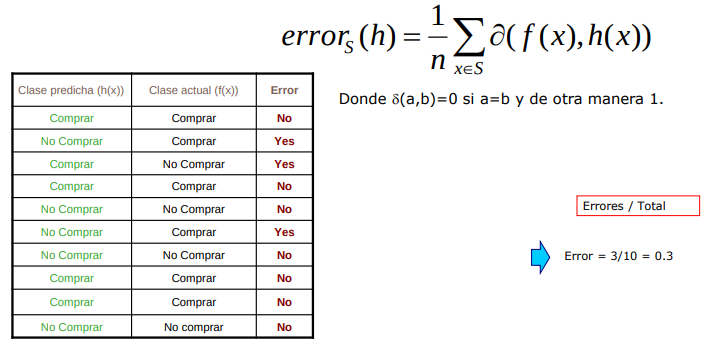
\includegraphics[scale=.65]{images/mod02-01.png}
\end{center}
En el ejemplo, el modelo desplegado, a través de los datos etiquetados como \ti{se ha comprado} o \ti{no se ha comprado} un producto, se comparan con los que predice el modelo. Vemos que en algunos casos no concuerdan, esos casos son \tb{errores}. En la clasificación lo que contamos es cuantas veces se falla, nos estamos refiriendo al \ti{error}; en el ejemplo las veces que falla la predicción son 3 sobre 10, el error es de \nperc{30} o \ti{0.3}. Podemos referirnos de forma inversa y decir que se acierta un \nperc{70} de las predicciones, lo que normalmente se llama \tb{porcentaje de acierto}, en inglés se desgina con el término \tb{accuracy}.

Este tipo de medida, porcentaje de acierto o porcentaje de error, es muy simple y en ocasiones se queda corta a la hora de entender como funciona realmente el modelo.

Una de las métricas habituales en clasificación son las que se conocen como:
\begin{itemize}
    \item \tb{Precission},  representa el porcentaje de documentos que son relevantes para la consulta, con \tb{TP} no referimos a \tb{True Positives}, \ti{valores positivos que han sido verdaderos}, en el ejemplo $TP/ \text{positivos predichos}$.
    ..
    \item \tb{Recall}, representa el porcentaje de documentos que se devuelven por el estudio o modelo (TP ), $TP/ \text{positivos reales}$.
\end{itemize}

Si queremos integrar estados medidas, que nos dé más información, podemos recurrir otro tipo de medida, también habitual que se denomina \tb{Medida F}, o también denominada \tb{media armónica}:

$$\text{Medida F} = 2\,\frac{\text{precission }\ast \text{ recall}}{\text{precission }+ \text{ recall}} = \frac{2TP}{2TP + FP + FN}$$

Un modelo con una \ti{Medida F} alta suele tener medidas altas en precission y recall.

\begin{description}
    \item[TP] o Positivos Predichos correctamente.
    \item[FP]  o Negativos Predichos como Positivos.
    \item[TN] o Negativos Predichos correctamente. 
    \item[FN] o Positivos Predichos como Negativos.  
    \item[TNRate] o porcentaje de negativos verdaderos 
\end{description}
estos parámetros nos permiten conocer el rendimiento de un modelo de clasificación binaria en circunstancias específicas.
\begin{center}
    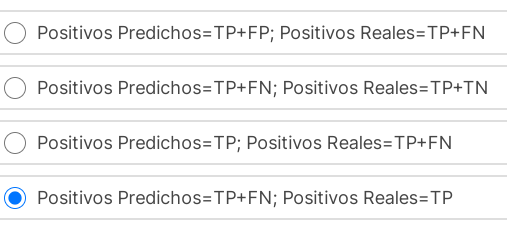
\includegraphics[scale=.65]{images/mod02-02.png}
\end{center}


\section{Métricas para regresión}

Recordemos que los modelos de regresión predicen un valor numérico a partir de una serie de entradas, este valor numérico no es algo exacto, sino que tiene decimales, en ocasiones muchos. Puesto que utiliza gran cantidad de datos, éstos pueden contener \ti{«ruido»} que hace que sea difícil obtener un valor exacto para la variable de salida.

Si quisieramos predecir la edad de una persona es una tarea difícil, lo que nos interesa es que los valores que obtengamos no se alejen mucho del valor real. Para evaluar cuánto nos alejamos o acercamos a ese valor real existen difrentes aproximaciones, que vemos a continuación, y se fundamentan en el cálculo del \tb{valor absoluto}, entre \ti{valor real} y el \ti{valor predicho}:

\begin{description}
    \item[Error Medio Absoluto, \funcc{MAE_S}{h}], lo que se hace es evaluar si el valor real menos el predicho, valor absoluto, para cada uno de los ejemplos de la muestra.
    $$\funcc{MAE_S}{h} = \frac{1}{n}\,\sum_{n\in S}|\func{x} - \funcc{h}{x}|$$
    \item[Error Cuadrático Medio, \funcc{MSE_S}{h} ],  lo que queremos es penalizar más aquellos casos en los que el error es más grande, lo que desequilibra el valor real del error, donde hay ejemplos que tienen un error pequeño y otros que puede ser enorme; utilizamos el \tb{error cuadrático}, consiste en elevar al cuadrado la diferencia entre el valor real y el predicho para cada uno de los ejemplos y calculamos su media.
    $$\funcc{MSE_S}{h} = \frac{1}{n}\,\sum_{n\in S}(\func{x} - \funcc{h}{x})^2$$
    Con este cálculo un error de 5 unidades se transforma en 25, pero uno de 10 se convierte en 100.
    \item[Raíz Cuadrada del Error Cuadrático Medio, \funcc{RMSE_S}{h}] , es un método que se utiliza para ajustar el valor que obtuvimos con \funcc{MSE_S}{h} a algo más real, consiste en obtener la \tb{ráiz cuadrada}. En ocasiones se confunden estos dos últimos cálculos, y no se distingue cuál se utiliza hasta que no se ven los cálculos realizados.
    $$\funcc{RMSE_S}{h} = \sqrt{\funcc{MSE_S}{h}} = \sqrt{ \frac{1}{n}\,\sum_{n\in S}(\func{x} - \funcc{h}{x})^2 }$$
\end{description}

Veamos un ejemplo, tenemos valores predichos y actuales (reales) para diez ejemplos:
\begin{center}
    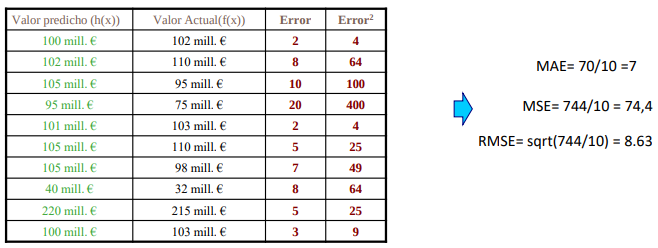
\includegraphics[scale=.65]{images/mod02-03.png}
\end{center}

Ignoraremos los millones y calculamos el \tb{error}, valor abosluto, como la diferencia entre valor actual y valor predicho, se suman todos estos valores obtenidos de error y se dividen por el número de ejemplos y obtendremos el valor de \funcc{MAE}{h} = 7. Por otra parte, el error cuadrático medio lo que hace es elevar al cuadrado cada uno de los valores obtenidos para el error, valor absoluto, y calcula la media, obteniendo un valor de \funcc{MSE_S}{h} de 74,4, como vemos al elevar al cuadrado, algunos de los errores son muy elevados, lo que dificulta la comparación ambos valores. Por último, para corregir esto recurrimos a calcular la ráiz cuadrada de \funcc{MSE_S}{h}, $\funcc{RMSE_S}{h} = \sqrt{74,4} = 8,63$.

¿Qué media se utiliza más?. En principio el \funcc{MSE_S}{h}, penaliza más los errores, más grandes, fijándonos en el caso de valor 400, es más de la mitad de la suma de todos los cuadráticos, no contribuye a la media de todo el error cuadrático, lo que penaliza la métrica muchísimo más.

Con el valor del \ti{error cuadrático medio} podemos ver los valores que detecta bien esos valores. Mediante la \ti{raíz cuadrada} obtenemos un valor expresado en términos de la magnitud.

Podemos tener un modelo en que los valores alrededor de mil, y casi todos los ejemplos son mil uno, novecientos noventa y nueve, \ldots, es decir, que si yo tengo un error de tres, porporcionalmente es pequeño, tres entre mil es muy pequeño, pero en realidad si los valores reales están entre mil uno, mil dos, novecientos noventa y nueve, el error que cometo es muy alto, la variabilidd que tiene esos datos es tan pequeña que el error es mucho más grande que la variabilidad o por eso normalmente las métricas de error relativo lo que hacen es dividir por algo que mida más o menos la variabilidad. La forma de medir esta variabilidad es utilizando las \tb{varianzas}:

\begin{description}
    \item[Error Cuadrático Medio Relativo]
    $$ \funcc{RSE_S}{h} = \frac{ \displaystyle{\sum_{n\in S}(\func{x} - \funcc{h}{x})^2 }}{\displaystyle{\sum_{x\in S}(\overline{f} - \func{x})^2}} $$
    \item[Error Absoluto Medio Relativo]  
    $$ \funcc{RAE_S}{h} = \frac{ \displaystyle{\sum_{n\in S}|\func{x} - \funcc{h}{x}|}}{\displaystyle{\sum_{x\in S}|\overline{f} - \func{x}|}} $$
\end{description}

Una medida fácil de calcular y que permite ver si el mdodelo es alto cuando el valor real es alto y bajo cuando el valor real es bajo, es calcular la correlación:
\begin{itemize}
    \item \tb{Correlación de Pearson}, que es la correlación lineal.
    \item \tb{Correlación de Spearman}, correlación de rangos o de orden.
\end{itemize}

\subsection{Métricas para Aprendizaje No Supervisado}

Una de las tareas más habituales en \ti{aprendizaje no supervisado} es el \tb{agrupamiento} o \tb{clustering}; lo que queremos obtener con el agrupamiento, donde tenemos un conjunto de datos y en el que no hay variables de salida, sólo de entrada, es separar los ejemplos que tienen relación entre sí y forman un grupo, de los que se diferencian y pertenecen a otros grupos. La idea es la diferencia o similitud en términos de distancia, se trata de una \ti{métrica de distancia}. Para ver que elementos son diferentes, establecemos si la distancia entre elementos es alta.

¿Cómo creamos estos grupos? . Podemos crear grupos donde los elementos que los integran estén muy cerca, a poca distancia, y que están muy lejos unos grupos de otros. Esto dependerá de la técnica que utilicemos para el agrupamiento, no todas las técnicas hacen el agrupamiento de la misma forma.

Por ejemplo, si utilizo una técnia de agrupamiento que me saca bordes en los grupos, lo que me puede interesar es establecer la distancia entre los \ti{«bordes de los clusters»} o entre los \ti{elementos más extremos}, pero puede interesarme establecer la distancia entre los centros de dos grupos para ver si están lejos o no. Por lo tanto, podemos mirar un \ti{centroid, el radio, lo grande que son los clusters,\ldots}, noes compleja la evaluación de elementos de los modelos de agrupamiento, pero hay muchas métricas, dependiendo de si queremos más separación, que estén mas compactos.

\begin{center}
    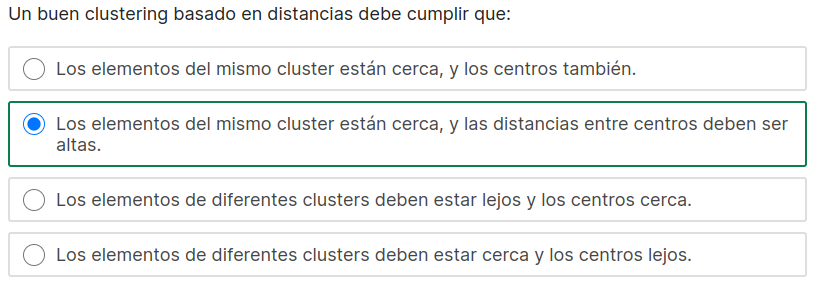
\includegraphics[scale=.65]{images/mod02-04.png}
\end{center}

\subsection{Sobreajuste}

Pensemos en un modelo de regresión en el que queramos evaluar la edad o las ventas dependiendo del mes,  si disponemos del \ti{error cuadrático medio} o el \ti{error absoluto}, lo que necesitamos es extraer el menor error posible. Es relativamente fácil, si disponemos de unos datos, ajustar esos datos de forma que minimizen el error, pero si luego lo utilizamos con otros datos, el mismo modelo, puede que no se ajuste igual de bien.

El típico ejemplo de \tb{sobreajuste}, que todos vivimos como estudiantes al estudiar un exámen anterior real, nos hemos ajustado a las preguntas que salian en él, pero cuando hacemos el exámen real, las preguntas han cambiado, y el resultado no ha sido lo bueno que esperabamos. Es un caso típico de \ti{sobreajuste} que aparece en el \ti{«aprendizaje humano»}, en el \ti{aprendizaje automático} aparece exáctamente los mismo; si entrenamos un modelo a partir de unos datos y lo evaluamos sobre esos datos es fácil engañarse, es muy fácil ajustarse a esos datos y cuando tengamos otros datos desconocidos fallemos. Podemos verlo reflejado gráficamente como:
\begin{description}
    \item[Over-fitting o sobreajuste], utilizamos todos los datos para entrenar y evaluar los modelos. Gráficamente uniriamos todos los puntos, como cuando hacemos un dibujo., pero no generalizamos en las zonas en las que estén cerca esos puntos
    \begin{center}
        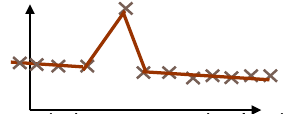
\includegraphics[scale=.65]{images/mod02-05_1.png}
    \end{center}
    En la gráfica vemos un pico, que se correspondería con un error o porque los datos en esa zona tienen una cierta variabilidad e intentamos un ajuste a algo que realmente no es un patrón de datos. Lo que deberíamos haber hecho es seguir la línea y evitar el pico.
    \item[Under-fitting o subajuste], compensamos el modelo generalizándolo, el ejemplo sería \ti{podar un árbol de datos}
    \begin{center}
        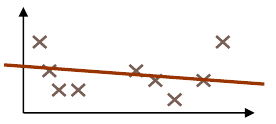
\includegraphics[scale=.65]{images/mod02-05_2.png}
    \end{center}  
    Viendo la gráfica podríamos pensar que los datos tienen un cierto patrón o contínuo entre los puntos representados, que podría intentar ajustar, pero no lo hacemos. Hemos generalizado demasiado el modelo con lo que prácticamente no obtenemos ningún patrón.
\end{description}

Esta es la duda principal, cómo puedo resolver o distinguir entre ambos casos automáticamente o visualmente. Lo que haremos es lo que se denomina \tb{regla de oro de la evaluación}:
\begin{center}
    \tb{\ti{nunca usar el mismo ejemplo para entrenar el modelo y evaluarlo}}
\end{center}
La mejor forma de hacer esto es escoger un conjunto de datos y separarlos o disponer de dos conjuntos diferentes de datos y utilizar un conjunto para el entrenamiento y el otro para la evaluación. En la práctica lo que haremos srá coger los datos y los dividiremos entre datos de entranamiento y datos para test.
\begin{center}
    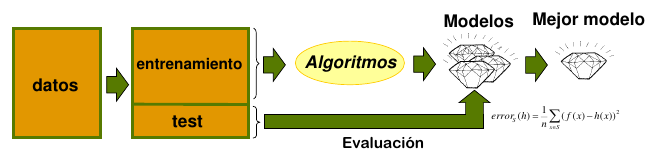
\includegraphics[scale=.65]{images/mod02-06.png}
\end{center}
¿Cuántos cogemos para entrenamiento y cuántos para el test? Variará dependiendo del experimento, pero suele ser $2/3$ para entrenamiento y $1/3$ para test, o $70:30$.

¿Cómo se hace esta separación?. No se hace en orden, sino  de forma aleatoria; no se hace en el orden en que se reciben los datos ya que pueden tener algún tipo de sesgo, se hace un muestreo aleatorio, donde extraemos el \nperc{70} de los datos para entrenamiento y el resto para el la evaluación.

En el \ti{entrenamiento} lo que hacemos es aplicar los \tb{algoritmos} y \tb{obtener modelos}, que constitiye la parte central del aprendizaje automático. Una vez obtenidos los modelos los \tb{evaluamos} con los datos de test, con ello podremos empezar a calcular las métricas o lo que sea necesario. En ese caso sabemos que si el modelo se hubiera ajustado a particularidades, que por casualidad han caído en los datos de entrenamiento o intenta ajustarse mucho al \ti{«ruido»} de esos datos, variabilidades que puedan presentar los datos, cuando se entra en la fase de test, eso se notará, el modelo tendrá peores resultados en la evaluación. Con eso podremos resolver el \ti{sobreajuste} y el \ti{subajuste}, al final la medida que tenemos que mirar es  la \ti{medida que nos den los datos de la evaluación}.

¿Y la \tb{cohesión}?. Hemos dividido los datos en la proporción \ti{70:30}, imaginemos que tengo cien datos, puedo pensar ¿por qué no entreno con los 100 datos?, si 100 datos son pocos y ahora los divido en dos grupos (\ti{70:30}), pierdo un \nperc{30} de datos en el entrenamiento y tan sólo utilizo 30 ejemplos para evaluar el modelo. La solución no es aumentar el porcentaje de datos para entrenamiento, ésto hace que siga disminuyendo el número de datos para evaluar el modelo, el balance entre datos de entrenamiento y de test es difícil de encontrar, sobre todo cuando el volumen de datos es pequeño.

Cuantos más ejemplos tengamos para entrenamiento y test mejor, pero siempre sin romper la \ti{regla de oro}. Si no queremos un entrenamiento y evaluación pobres, y tenemos pocos datos, la solución se basa en la \tb{repetición del experimento}, varias veces sin romper en cada uno de los experimentos la \ti{regla de oro}, y al final hacer \tb{promedios de los resultados} obtenidos en cada experimento. Hay bastantes  maneras de hacerlo, pero nos centramos en dos:
\begin{itemize}
    \item \tb{Bootstrap}, se cogen n-muestras con repeticiones y se realiza la evaluación con el resto, se obtienen ejemplos con repetición, un ejemplo puede salir varias veces, y luego se testea con el resto. No se sigue ningún orden.
    \item \tb{Validación cruzada}, particionamos los datos en lo que se llaman \tb{pliegues}, evaluamos con un pliegue y aprendemos con el resto de ejemplos.
\end{itemize}

\subsection{Validación Cruzada}

En un contexto donde tengamos muchos datos, el problema de los datos de entrenamiento y de evaluación no sería un problema, dispondríamos de datos suficientes para aplicar la \ti{regla de oro}, pero en los casos en que tenemos pocos datos (100, 200, \ldots) tenemos un dilema, al dividirlos en datos de entrenamiento y de validación, tendríamos pocos casos para ambos grupos, por lo tanto, hemos de intentar resolver este problema.

Existe una solución, que a base de aplicar repetición podemos conseguir no romper la \ti{regla de oro}. ¿Cómo conseguir este proceso mágico?. Es un proceso que se conoce como \tb{validación cruzada}, en principio, tenemos los datos que partiremos en \ti{n-pliegues},
\begin{center}
    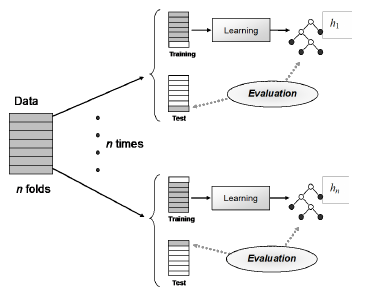
\includegraphics[scale=.67]{images/mod02-07.png}
\end{center}
en la imagen vemos que se han creado 7 pliegues, quiere decir que por cada iteración tendremos siete iteraciones, en la imagen sólo vemos la primera y la última; en cada iteración cogeremos uno de los pliegues para test, evaluación del modelo, y el resto para entrenamiento, esto se hará siete veces. A continuación, lo que se hace es sencillo, cogemos los seis pliegues de entrenamiento, cada pliegue puede tener 10, 15, \ldots ejemplos, los que hayan salido y entrenar el modelo y, por último, evaluarlo con el pliegue destinado a test.

Supongamos que tras el proceso obtenemos un \nperc{93} en el primero de los pliegues. En el pliegue dos podríamos obtener un \nperc{92.5}, así con el resto de pliegues, y el último podría ser de \nperc{94.2}. Hacemos un promedio de esos valores, que podemos suponer que sea de \nperc{92.7}, con ese promedio, que es el de \ti{evaluación}, indicaría cómo se comporta el modelo. Lo siguiente sería determinar con cuál de los grupos (pliegues) nos quedamos, y a cuál de ellos asigno el promedio estimado. La respuesta es \tb{a ninguno}. Lo que haríamos, que no refleja la imagen, es escoger todos los datos y entrenamos el modelo con todos esos datos, el resultado, en este ejemplo que hemos supuesto que era de clasificación, es un \tb{árbol de decisión} que se comporta como la media de todos los otros modelos que entrenamos en su momento, que era \nperc{93.7}, lo que hacemos es quedarnos con el modelo que acabamos de entrenar, con todos los datos y le asignamos una evaluación de \nperc{93.7}. ¿Por qué establecemos ésta canlidad? Si nos fijamos, todos los modelos se han evaluado sólo con seis pliegues, pero el último modelo lo hemos generado con todos los pliegues, el conjunto de datos inicial, con lo que tenemos más datos, lo que hace que el modelo obtenido es mejor, suele ser una estimación más robusta y, además, conseguimos entrenar el modelo con todos los datos. Si nos fijamos, en ningún momento hemos evaluado con datos que se utilizaron para el entrenamiento.

Normalmente, en este método de \ti{variación cruzada} es habitual utilizar diez pliegues, pero depende del coste computacional, cada pliegue son repeticiones, si hay diez pliegues, son diez repeticiones más el modelo final, es decir, \ti{once procesos de aprendizaje}. Si se trata de una tarea costosa como puede ser una red neuronal, podemos limitar esos pliegues a cinco o cuatro, pero si no son muchos los datos, que es cuando realmente utilizamos la \ti{variación cruzada}, podemos irnos a 10, 20 o incluso hacer tantos pliegues como ejemplos, en el caso de que los recursos nos lo permitan y tengamos pocos ejemplos.

\begin{center}
    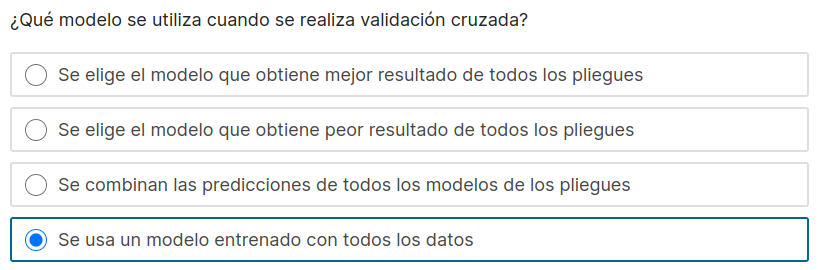
\includegraphics[scale=.67]{images/mod02-08.png}
\end{center}

Hemos visto que los modelos de \ti{clasificación} se suelen evaluar con métricas relacionadas con el \ti{porcentaje de acierto}, mientras que las tareas de regresión se evalúan con métricas relacionadas con el \ti{error absoluto medio} o el \ti{error cuadrático medio}. Lo que no sabemos es dónde falla exactamente nuestro modelo. Para ello, vamos a ver para la \ti{clasificación} y la \ti{regresión} dos formas de representar cómo se manifiestan esos errores, como se distribuyen:
\begin{itemize}
    \item \ti{Clasificación}, veremos la \tb{contingencia}, cómo se distribuyen los errores, también se denomina \tb{confusión} o \tb{matriz de confusión}.
    \begin{center}
        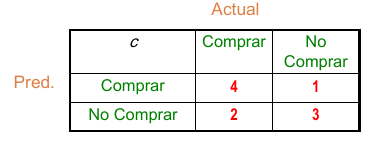
\includegraphics[scale=.67]{images/mod02-09.png}
    \end{center}
    Esta matriz que representa un problema de dos clases: comprar o no comprar, quiere predecir si un cliente compra o no compra un producto. Suponemos que tenemos diez ejemplos, de ellos, si vemos la parte superior (Actual) representa los valores reales, tendremos $4+2=6$ en la primera columna, seis casos reales en los que el cliente compró, y $1+3=4$ en los que no compró. Lo que queremos ver es si nuestro modelo \ti{predice bien o no}.
    \begin{enumerate}
        \item Podemos ver que realmente acierta siete veces, 4 se predicen como de compra y 3 como de no compra. Pero queremos saber su distribución, ¿cuántos de los que realmente se compró, van a parar a parar a no comprar y cuántos de los que no se compró, van a compró?, es decir, la otra diagonal de la tabla, la \ti{diagonal de los errores}. Podemos ver que de los 6 que se compraron, en 4 acierta el modelo y en dos falla, y de los que no compraron, 1 falla y 3 acierta; vemos cláramente como se distribuye. Vemos que de los 6 casos de comprar, acierta 4 y falla 2 que representa una tercera parte, y de los no compra, 4 ejemplos, falla 1 y acierta 3, una cuarta parte, por lo tanto, los errores parecen estar bien balanceados.
    \end{enumerate}
    \item \ti{Regresión}, en lugar de una matriz de 2,3, n-clases lo que tenemos es un número, en principio, infinito de valores y no podemos representarlos en una clase. Si predice $3.2$ y el valor real es $3.1$,  estamos bastante cerca, aunque si se hiciera como clasificación, serían casillas diferentes. Aquí lo que generaremos es un \tb{gráfico de dispersión} que representa en un eje el valor predicho y en el otro el actual (no importa en qué eje pongamos estos valores)
    \begin{center}
        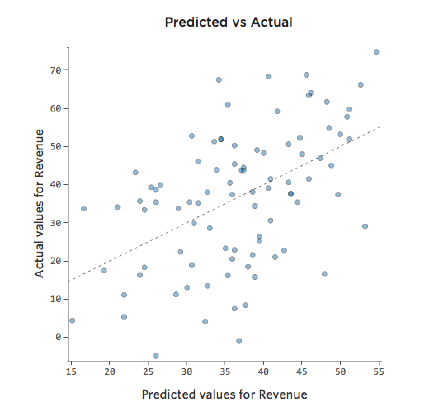
\includegraphics[scale=.67]{images/mod02-10.png}
    \end{center}
    Si tenemos un valor predicho de 40 podemos ver el valor real correspondiente, siendo $\approx 20.xxx$, en este ejemplo indica que el valor real es mucho menor que el predicho. Los valores por encima de la diagonal del gráfico nos indican valores predichos que se han quedado más cortos que el valor real , mientras que los que están por debajo se han alejado más. Dicha diagonal representa un \tb{clasificador perfecto},  y nos servirá para ver los casos de \ti{sobreajuste} y \ti{subajuste}, tendremos una visión bastante clara de cómo se distribuyen nuestros errores, tanto en clasificación como regresión.
\end{itemize}

Con estos procesos podemos comparar incluso distintas matrices de confusión o de contingencia y distintos gráficos de dispersión.

\begin{center}
    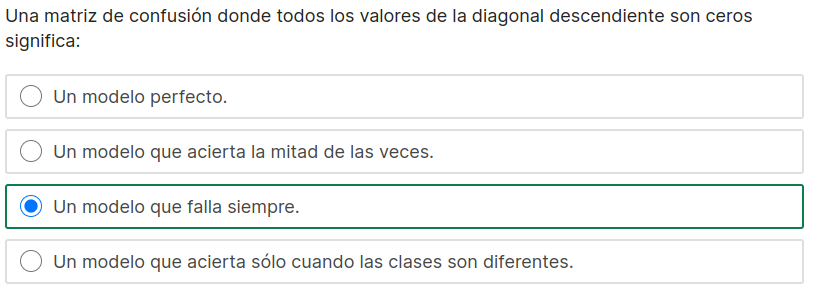
\includegraphics[scale=.67]{images/mod02-11.png}
\end{center}

\subsection{Clasificación binaria: Matriz de confusión}

De una matriz de contingencia o de confusión de un clasificador podemos extraer cualquier tipo de medida.

Si tenemos esta matriz de confusión, en la que tenemos los valores reales, son las columnas, y los valores predichos son las filas, estos serían los positivos verdaderos, los positivos falsos, que son errores, por eso son falsos, los negativos verdaderos que son aciertos y los negativos falsos.
\begin{center}
    \begin{tabular}{ c c }
        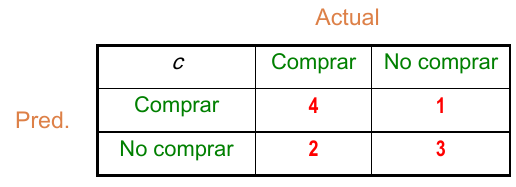
\includegraphics[scale=.67]{images/mod02-12_1.png}    &
        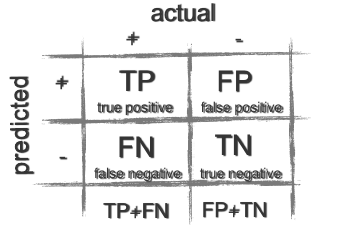
\includegraphics[scale=.67]{images/mod02-12_2.png}    
    \end{tabular}
\end{center}
En el ejemplo de comprar-no comprar